\documentclass[conference]{IEEEtran}
\IEEEoverridecommandlockouts
% The preceding line is only needed to identify funding in the first footnote. If that is unneeded, please comment it out.
\usepackage{amsmath,amsthm,amssymb} %modos matemáticos y  simbolos
\usepackage{latexsym,amsfonts} %simbolos matematicos
\usepackage{cancel} %hacer la linea que cancela las ecuaciones
\usepackage[spanish, es-noshorthands]{babel} %comandos en español y cambia el cuadro por la tabla
\decimalpoint %cambia las comas por puntos decimal
\usepackage[utf8]{inputenc} %caracteristicas del español
\usepackage{physics} %Simbolos fisicos
\usepackage{array} %mejores formatos de tabla
\parindent =0cm %sangria 
\usepackage{algorithmic}
\usepackage{graphicx}
\usepackage{textcomp}
\usepackage{xcolor}
\usepackage{mathtools} 
\usepackage[framemethod=TikZ]{mdframed}%Entornos talegas
\usepackage[colorlinks = true,
			linkcolor = blue,
			citecolor = black,
			urlcolor = blue]{hyperref}%formato de los links y URL's
\usepackage{multicol} %varias columnas
\usepackage{enumerate} %enumeraciones
\usepackage{pgf,tikz,pgfplots} %documentos en formato tikz
\usepackage{mathrsfs} %letras chingonas (transformada de laplace)
\usepackage{subfigure} %varias figuras seguidas
\usepackage{tabulary}
\usepackage{multirow} %ocupar varias filas en una tabla
\usepackage{fancybox} %recuadros talegas
\usepackage{float} %ubicar graficas
\usepackage{color}
\usepackage{comment}
\usepackage{stackrel}
\usepackage{calligra}
\usepackage{lipsum}
\usepackage{cite}
%\pgfplotsset{compat=1.17} 

\newcommand{\R}{\mathbb{R}}
\newcommand{\Z}{\mathbb{Z}}
%%%%%%%%%%%%%%%%%%%%%%%%%%%%%%%%%%%%%%%%%%%%%%%%%%%%%%
\def\BibTeX{{\rm B\kern-.05em{\sc i\kern-.025em b}\kern-.08em
    T\kern-.1667em\lower.7ex\hbox{E}\kern-.125emX}}
\begin{document}



%%% CARÁTULA
\begin{titlepage}



\begin{flushleft}
    Universidad de San Carlos de Guatemala \\
    Escuela de Ciencias Físicas y Matemáticas \\
    Curso: Laboratorio de Instrumentación \\
    Profesor: Wendy Miranda
\end{flushleft}

\vspace{8cm}

\begin{center}
    \huge{Parcial 2}
\end{center}

\vspace{10cm}

\begin{flushright}
    Diego Sarceño \\
    $201900109$
\end{flushright}

\vspace{0.5cm}

\begin{center}
    Guatemala, 16 de noviembre del 2022
\end{center}

\end{titlepage}



\section{Problema 1}
Para este problema se tienen los siguientes datos: Ganancia de voltaje $A_v = -25$, corriente máxima por los resistores $I = 10\mu A$ y el voltaje de entrada $V_I \in [-25,25]mV$. Dada la corriente máxima y el voltaje de entrada podemos encontrar las resistencias mostradas en la figura \ref{p1}, sabiendo que la corriente es la misma en ambas
	$$ R_1 = \frac{V_I}{I} = \boxed{ 2.5k\Omega , } $$
	$$ R_2 = \abs{-R_1 A_v} = \boxed{ 62.5k\Omega . } $$


\begin{figure}[H]
	\centering
	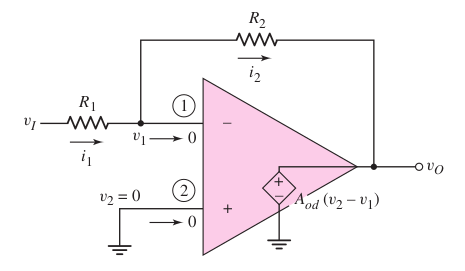
\includegraphics[scale=0.4]{img/p1.png}
	\caption{Problema 1.}
	\label{p1}
\end{figure}

Además, teniendo la ecuación $A_v V_I = V_o$ para el voltaje de salida, encontramos el rango de voltajes
	$$ \boxed{ V_o \in [-625,625]mV . } $$
\\
\section{Problema 2}
Dado el voltaje de salida del circuito inversor sumador (Figura \ref{p2}) $ V_o = -3 \qty( V_{I1} + 2V_{I2} + 0.3V_{I3} + 4V_{I4} ) $ y que la resistencia máxima es de $400k\Omega$.

\begin{figure}[H]
	\centering
	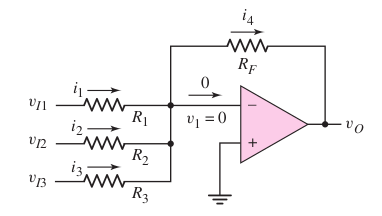
\includegraphics[scale=0.5]{img/p2.png}
	\caption{Problema 2.}
	\label{p2e}
\end{figure}

Dado que $400k\Omega$ es la resistencia máxima, y la razón $\frac{R_F}{R_3} = 0.9$ es menor a $1$, tomamos $\boxed{ R_3 = 400k\Omega }$. Con el voltaje de salida se tiene la siguiente igualdad
	$$ -\qty( 3V_{I1} + 6V_{I2} + 0.9V_{I3} + 12V_{I4} ) =  $$
	$$ -\qty(\frac{R_F}{R_1} V_{I1} + \frac{R_F}{R_2} V_{I2} + \frac{R_F}{R_3} V_{I3} + \frac{R_F}{R_4} V_{I4} ), $$
entonces
	$$ \boxed{ R_F = 360k\Omega , } \qquad \qquad \boxed{ R_1 = 120k\Omega , } $$
	$$ \boxed{ R_2 = 60k\Omega , } \qquad \qquad \boxed{ R_4 = 30k\Omega . } $$

Dando valores a los voltajes de entrada
\begin{enumerate}[i)]
	\item $V_{I1} = 0.1V$, $V_{I2} = -0.2V$, $V_{I3} = -1V$ y $V_{I4} = 0.05V$. Entonces, valuando en la ecuación dada del voltaje de salida
		$$ V_o = -3[(0.1) + (-0.2)(2) + (0.3)(-1) + (0.05)(4)] = \boxed{ 1.2V. } $$
	\item $V_{I1} = -0.2V$, $V_{I2} = 0.3V$, $V_{I3} = 1.5V$ y $V_{I4} = -0.1V$. Entonces, valuando en la ecuación dada del voltaje de salida
		$$ V_o = -3[(-0.2) + (0.3)(2) + (0.3)(1.5) + (-0.1)(4)] = \boxed{ -1.35V. } $$
\end{enumerate}
\vspace{0.3cm}

\section{Problema 3}
Para el voltaje de entrada, encontramos la pendiente de la recta entre $[0,5] \mu s$ (la cual solo cambia de signo para el tramo siguiente, y ahí se cumple un ciclo)
	$$ m = \frac{5V - (-5V)}{5\mu s - 0} = 2\times 10^6 V/s, $$
con esto, definimos la función periodica por tramos
	$$
		V_I (t) = \left\{\begin{array}{cc}
			\qty(2\times 10^6 V/s)t - 5V & \text{ de } \quad 0-5\mu s, \, 10-15\mu s, \, \ldots \\
			\qty(-2\times 10^6 V/s)t + 5V & \text{ de } \quad 5-10\mu s, \, 15-20\mu s, \, \ldots 
		\end{array}\right. .
	$$
Entonces, dada la ecuación 9.72 del libro \cite{b1}
	$$ V_o (t) = -R_2 C_1 \dv{V_I (t)}{t}, $$
valuando, se tiene el voltaje de salida
	$$ 
		V_o (t) = -R_2 C_1 \left\{\begin{array}{cc}
			2\times 10^6 V/s & \text{ de } \quad 0-5\mu s, \, 10-15\mu s, \, \ldots \\
			-2\times 10^6 V/s & \text{ de } \quad 5-10\mu s, \, 15-20\mu s, \, \ldots
		\end{array}\right. .
	$$
El cuál tiene límite superior $4.4V$ y límite inferior $-4.4V$. Además, dado esto, podemos graficar dicho voltaje, el cual son trozos de función constante iniciando en el límite inferior,
\begin{figure}[H]
	\centering
	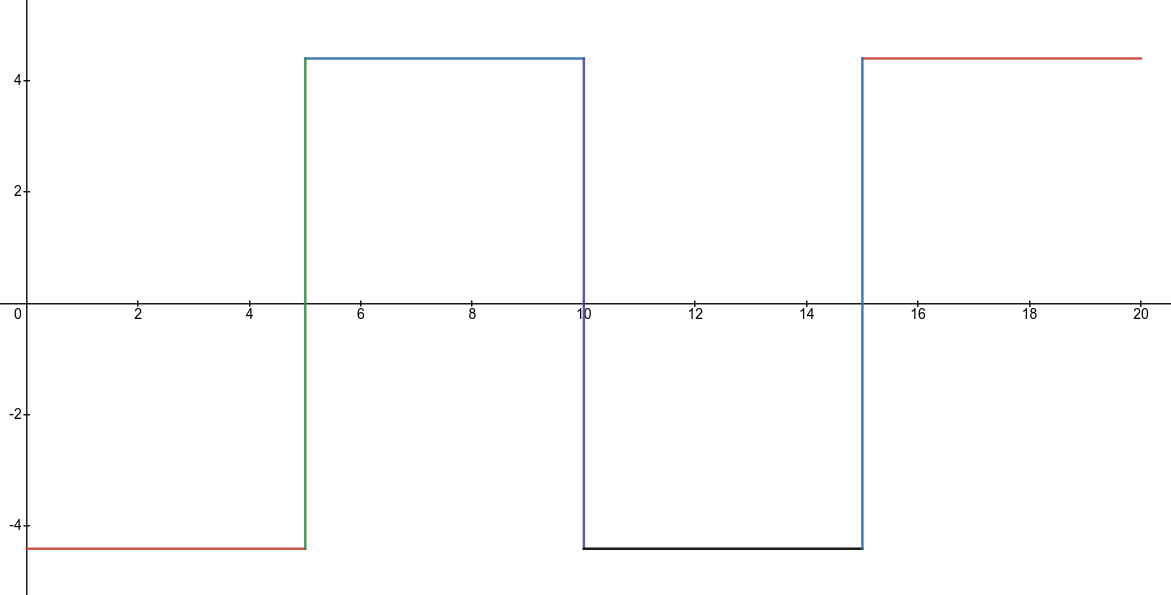
\includegraphics[scale=0.2]{img/p3g.png}
	\caption{Voltaje de salida, problema 3.}
	\label{p2e}
\end{figure}

\vspace{0.3cm}

\section{Problema 4}
Dado el circuito
\begin{figure}[H]
	\centering
	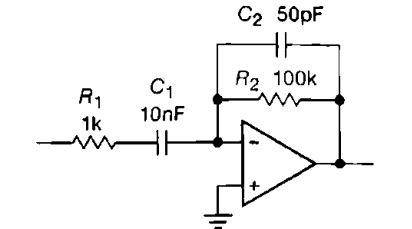
\includegraphics[scale=0.5]{img/p4.png}
	\caption{Problema 4.}
	\label{p2e}
\end{figure}

se tiene que la ganancia de voltaje es $A_v = -\frac{Z_2}{Z_1}$, donde las impedancias son
	$$ Z_1 = R_1 + \frac{1}{j\omega C_1} = \frac{1 + j\omega R_1 C_1}{j\omega C_1}, $$
	$$ Z_2 = \frac{\frac{R_2}{j\omega C_2}}{R_2 + \frac{1}{j\omega C_2}} = \frac{R_2}{1 + j\omega R_2 C_2}. $$
Con esto, encontramos la ganancia
	$$ A_v = \frac{-j\omega R_2 C_1}{(1 + j\omega R_1 C_1)(1 + j\omega R_2 C_2)}, $$	
entonces, por definición $A_v \frac{V_o}{V_I}$, se tiene
	$$ \boxed{ V_o = \frac{-j\omega R_2 C_1 V_I}{(1 + j\omega R_1 C_1)(1 + j\omega R_2 C_2)} } $$




%\begin{abstract}
%    
%\end{abstract}
%
%\begin{IEEEkeywords}
%    
%\end{IEEEkeywords}
%
%\section{Objetivos}
%
%\subsection{General}
%    \begin{enumerate}[1.]
%        \item 
%    \end{enumerate}
%\subsection{Específicos}
%    \begin{enumerate}
%        \item 
%    \end{enumerate}
%%\section{Introducción}
%    
%\section{Marco Teórico}
%    
%\section{Diseño Experimental}
%    \subsection{Materiales a Utilizar}
%        \begin{itemize}
%    	\item 
%    \end{itemize}
%
%    \subsection{Procedimientos}
%        \begin{enumerate}
%            \item 
%        \end{enumerate}
%\section{Resultados}
%    
%\section{Discusión de Resultados}
%\begin{enumerate}
%    \item 
%   
%\end{enumerate}
%\section{Conclusiones}
%\begin{enumerate}
%    \item 
%\end{enumerate}
%%\section{Recomendaciones}
%
%\section{Anexos}
%
\begin{thebibliography}{00}
\bibitem{b1} Neamen, D. A. (2007). \textit{Microelectronics: circuit analysis and design} (Vol. 43). New York: McGraw-Hill.
\end{thebibliography}

\end{document}